\chapter{Circuiti RLC}

\renewcommand\thesection{\Roman{section}}

\section{Rifasamento}

\textbf{Obiettivo:} minimizzare lo sfasamento tra tensione e corrente in un circuito RL tramite l'aggiunta in serie di un condensatore.

\paragraph{Strumentazione:}
\begin{enumerate}
    \item un generatore di funzioni;
    \item una resistenza;
    \item un induttore;
    \item un oscilloscopio.   
\end{enumerate}

\paragraph{Procedura:}
\begin{enumerate}
    \item costruire il circuito;
    \begin{figure}[h]
        \centering
        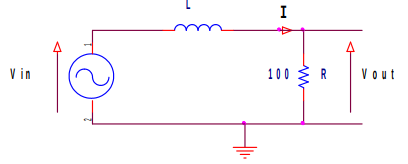
\includegraphics[width=0.6\linewidth]{Immagini/EXP4 - circuito RL.png}
        \caption{serie RL da rifasare.}
        \label{fig: EXP4 - circuito RL}
    \end{figure}
    \item misurare il valore di L e di Q (fattore di bontà);
    \item usando un generatore di funzioni applicare una tensione sinusoidale al circuito e con l'oscilloscopio visualizzare la tensione applicata all'ingresso e ai capi della resistenza. Si vede con i due canali dell'oscilloscopio che c'è uno sfasamento fra le due tensioni, ed anche fra tensione e corrente;
    \item con i cursori, misurare lo sfasamento tra le due tensioni;
    \item a partire dal valore misurato dell'induttanza, calcolare il condensatore necessario per il rifasamento ad una frequenza di circa 10 kHz;
    \item verificare che le due tensioni sono in fase misurando il loro sfasamento.
    \begin{figure}[h]
        \centering
        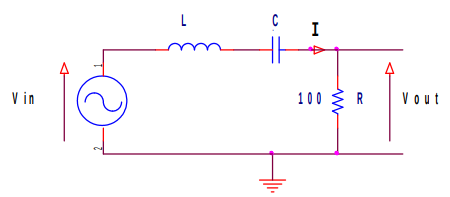
\includegraphics[width=0.55\linewidth]{Immagini/EXP4 - circuito RLC.png}
        \caption{serie RLC rifasata.}
        \label{fig: EXP4 - circuito RLC}
    \end{figure}
\end{enumerate}

\section{Guadagno di un soppressore di banda}

\paragraph{Obiettivo:} ricavare il guadagno di un soppressore di banda (o di un passa banda) in funzione della frequenza della tensione in ingresso.

\paragraph{Strumentazione:} 
\begin{enumerate}
    \item un generatore di funzioni;
    \item una resistenza;
    \item un induttore e un condensatore tali che la frequenza di risonanza $f_0$ sia di qualche kHz;
    \item un oscilloscopio.
\end{enumerate}

\paragraph{Procedura:}
\begin{enumerate}
    \item costruire il circuito;
    \begin{figure}[h]
        \centering
        \includegraphics[width=0.7\linewidth]{Immagini/EXP4 - passa|elimina banda.png}
        \caption{passa banda o soppressore di banda.}
        \label{fig: EXP4 - passa|elimina banda}
    \end{figure}
    \item collegare il generatore di funzioni, impostato su onde sinusoidali, all'ingresso del circuito;
    \item per eseguire la misura collegare un canale dell'oscilloscopio all'ingresso e l'altro all'uscita;
    \item per frequenze vicine a $f_0$ si avrà una tensione in uscita circa uguale a quella in ingresso (passa banda), oppure una tensione prossima a zero (soppressore di banda);
    \item caratterizzare la risposta del filtro in funzione della frequenza, misurando per ogni valore la tensione di ingresso e in uscita. Per caratterizzarlo al meglio, oltre a prendere misure nell'intorno di $f_0$, prenderne anche per valori di $f$ molto minori e molto maggiori di $f_0$;
    \item graficare il guadagno $A_V$ in funzione di $f$;
    \item verificare che cambiando il valore della resistenza del circuito la banda passante si restringe o si allarga;
    \item dopo aver ricavato mediante calcolo simbolico il guadagno in funzione di $f$, effettuare una regressione dei dati con la relativa funzione. Confrontare la frequenza di risonanza ottenuta dal fit con quella ricavabile dalle misure di L e C. Per l'inizializzazione dei parametri della funzione di fit utilizzare solo le informazioni ricavabili dai dati e non quelle su L e C. Dal fit estrarre il valore di $R_s$.
\end{enumerate}

\setcounter{section}{0}
\renewcommand\thesection{\Alph{section}}

\section{Corrente attraverso una serie RLC}
Se il generatore è di tipo sinusoidale si può applicare il metodo simbolico per il calcolo della corrente $I$ e si ottiene
\begin{equation}
  I = \frac{V_{in}}{R + j\omega L} = \frac{V_{in}}{R^2 + \omega^2 L^2}(R - j \omega L),
\end{equation}
da cui si ricava
\begin{equation}
    |I| = \frac{V_{in}}{\sqrt{R^2 + \omega^2 L^2}},\quad\tan{\phi}=\frac{-\omega L}{R},
\end{equation}
dove il segno meno indica che la corrente è in ritardo rispetto alla tensione. Per rifasare il circuito è necessario aggiungere un condensatore in serie ad $L$. La corrente diventa
\begin{equation}
I = \frac{V_{in}}{R + j\omega L - \frac{j}{\omega C}} = \frac{V_{in}}{R + j\left( \omega L - \frac{1}{\omega C} \right)}.
\end{equation}
Questa è in fase se $X_L=\omega L=1/(\omega C)=X_C$, da cui si può ricavare il valore di C. In questo caso l'impedenza $Z$ è puramente reale e resistiva.